\documentclass[varwidth=true, border=2pt]{standalone}

\usepackage{pgfplots}
\usepackage{tikz}

\usetikzlibrary{calc,patterns,angles,quotes}

\begin{document}
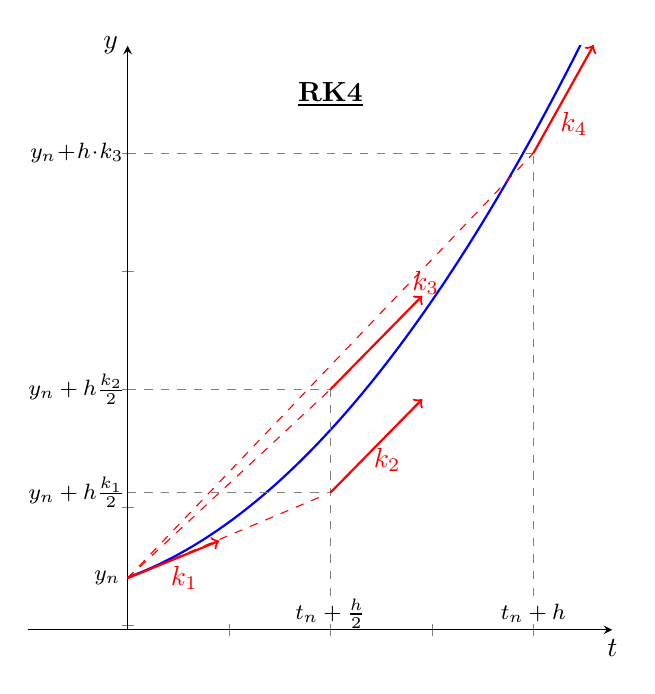
\begin{tikzpicture}
    \begin{axis}[
        legend pos=south east,
        axis x line=middle,
        axis y line=middle,
	every axis x label/.style={at={(current axis.right of origin)},anchor=north},
	every axis y label/.style={at={(current axis.above origin)},anchor=east},
	xticklabels=\empty,
	yticklabels=\empty
        grid = none ,
        width=9cm,
        height=9cm,
        grid style={dashed, gray!1},
        xmin=-0.25,     % start the diagram at this x-coordinate
        xmax=2.15,    % end   the diagram at this x-coordinate
        ymin=0.275 ,   % start the diagram at this y-coordinate
        ymax= 1.1,   % end   the diagram at this y-coordinate
        xlabel=$t$,
        ylabel=$y$,
        enlargelimits=true,
        tension=0.08]

        	\addplot[domain=0:2.25, blue, thick,samples=250] {0.125*(x+0.5)^2+0.25}; % Parabola
        	
	\addplot[dashed,red,mark=none] coordinates{(1,-0.15)(1,0.05)} node[below, pos=0] {}; %x1
	\addplot[dashed,gray,mark=none] coordinates{(2,0.25)(2,1)} node[below, pos=0] {}; %x1
	\addplot[dashed,gray,mark=none] coordinates{(1,0.25)(1,0.6)} node[below, pos=0] {}; %x1
	

	\addplot[dashed,gray,mark=none] coordinates{(0,0.6)(1,0.6)} node[below, pos=0] {}; %x1
	\addplot[dashed,gray,mark=none] coordinates{(0,0.425)(1,0.425)} node[below, pos=0] {}; %x1
	\addplot[dashed,gray,mark=none] coordinates{(0,1)(2,1)} node[below, pos=0] {}; %x1
	
	\draw [thick,red, <->] (axis cs: 1, -0.15) to (axis cs: 2.25, -0.15);
	
	\node(K1a) at (axis cs: 0,0.28){};
	\node(K1b) at (axis cs: 0.5,0.35){};
	\node(K2a) at (axis cs:1,0.425){};
	\node(K2b) at (axis cs:1.5,0.6){};
	\node(K3a) at (axis cs:1,0.6){};
	\node(K3b) at (axis cs:1.5,0.775){};
	\node(K4a) at (axis cs:2,1){};
	\node(K4b) at (axis cs:2.325,1.2){};
	\node(K4c) at (axis cs:2,1.05){};	
	
	\node(RK4) at (axis cs:1,1.1){\textbf{\underline{RK4}}};
	\node(TY) at (axis cs:-0.1,0.28){\footnotesize{$y_n$}};
	\node(YK1) at (axis cs:-0.25,0.425){\footnotesize{$y_n +h \frac{k_1}{2}$}};
	\node(YK2) at (axis cs:-0.25,0.6){\footnotesize{$y_n +h \frac{k_2}{2}$}};
	\node(YK3) at (axis cs:-0.25,1){\footnotesize{$y_n \! + \!  h\! \cdot \! k_3$}};
	\node(h1) at (axis cs:1,0.22){\footnotesize{$t_n + \frac{h}{2}$}};	
	\node(h2) at (axis cs:2,0.22){\footnotesize{$t_n +h$}};	
	
	
	\node(k1)[red] at (axis cs: 0.28,0.28){$k_1$};
	\node(k2)[red] at (axis cs: 1.28,0.48){$k_2$};	
	\node(k3)[red] at (axis cs: 1.47,0.78){$k_3$};	
	\node(k4)[red] at (axis cs: 2.2,1.05){$k_4$};	
	
	\draw [thick,red, <-] (K1b) to (K1a.center);
	\draw [dashed,red] (K1a.center) to (K2a);
	\draw [thick,red, ->] (K2a.center) to (K2b);
	\draw [dashed,red] (K1a.center) to (K3a.center);
	\draw [thick,red, ->] (K4a.center) to (K4b);
	\draw [dashed,red] (K1a.center) to (K4a.center);
	\draw [thick,red, ->] (K3a.center) to (K3b);
    \end{axis}
\end{tikzpicture}
\end{document}